\section{Dataset}

\begin{frame}{Dataset}
  \begin{columns}[T,onlytextwidth]
    \column{.46\textwidth}
      \footnotesize
      \textbf{RRDataset} — $\sim$51{,}000 images across 3 processing categories $\times$ 2 classes:
      \vspace{.25em}
      \centering
      \begin{tabularx}{\linewidth}{@{}Xrr@{}}
        \toprule
        Category & AI & Real \\
        \midrule
        Original            & 8500 & 8500 \\
        Transfer            & 8500 & 8500 \\
        Re-digitized        & 8500 & 8499 \\
        \bottomrule
      \end{tabularx}

      \vspace{.35em}
      \raggedright
      \begin{itemize}
        \item Balanced sampling per class (default 6000/class), fixed seed.
        \item \textbf{Leakage-safe split}: images grouped by parent photo ID before the 80/10/10 split, so a processed photo never lands in a different split than its original.
        \item Labels: Real/Fake (\texttt{ai=0}, \texttt{real=1}), Transform (\texttt{original=0}, \texttt{transfer=1}, \texttt{redigital=2}).
      \end{itemize}

    \column{.50\textwidth}
      \centering
      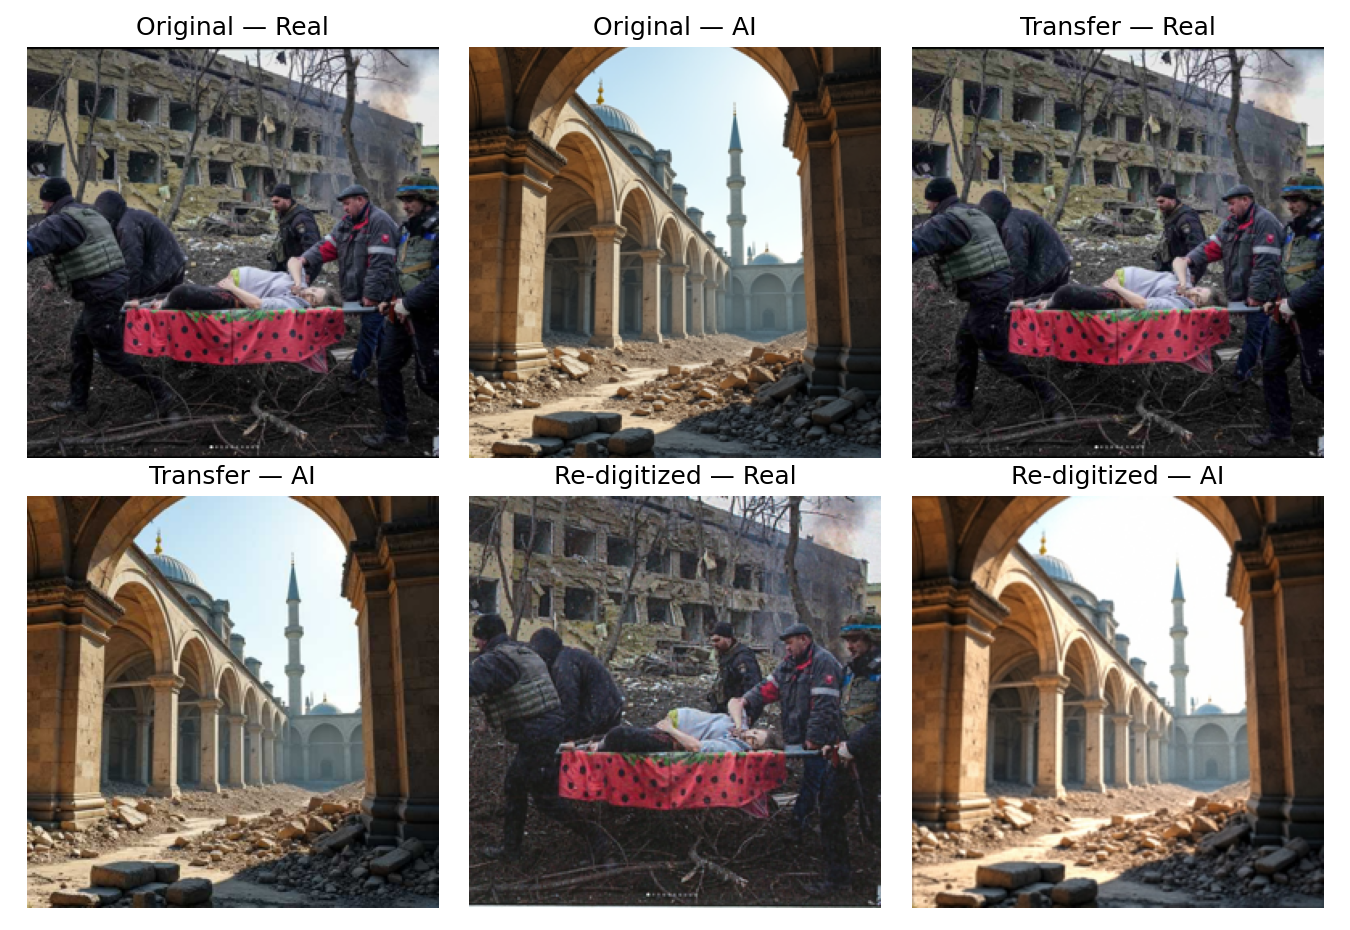
\includegraphics[width=\linewidth]{assets/dataset_samples.png}\\
      {\footnotesize\color{cookieMuted} One sample per (category $\times$ real/fake) cell}
  \end{columns}
\end{frame}
